\documentclass[11pt]{article}
\usepackage{amsmath, amssymb, amscd, amsthm, amsfonts}
\usepackage{graphicx}
\usepackage{hyperref}

% Korean packages
\usepackage[T1]{fontenc}
\usepackage{CJKutf8}

\oddsidemargin 0pt
\evensidemargin 0pt
\marginparwidth 40pt
\marginparsep 10pt
\topmargin -20pt
\headsep 10pt
\textheight 8.7in
\textwidth 6.65in
\linespread{1.2}

\title{Tverberg's theorem is 50 years old\\
	\large MATH 818.01 Midterm Survey
}
\author{Hyungkuk Yoon}
\date{}

\newtheorem{theorem}{Theorem}
\newtheorem{lemma}[theorem]{Lemma}
\newtheorem{conjecture}[theorem]{Conjecture}

\newcommand{\rr}{\mathbb{R}}

\newcommand{\al}{\alpha}
\DeclareMathOperator{\conv}{conv}
\DeclareMathOperator{\aff}{aff}

\begin{document}
	
	\maketitle
	
	\begin{abstract}
		This survey presents an overview of the advances around Tverberg's theorem, focusing on the last two decades.  We discuss the topological, linear-algebraic, and combinatorial aspects of Tverberg's theorem and its applications.  The survey contains several open problems and conjectures.
		\begin{CJK}{UTF8}{mj}
			한글도 사용 가능합니다.
		\end{CJK}
	\end{abstract}
	
	\section{Introduction}\label{section-introduction}
	
	\begin{CJK}{UTF8}{mj}
		본문에서도 당연히 한글 사용 가능합니다..만, CJK 환경으로 지정해야 합니다. 텍 소스를 보세요.
	\end{CJK}
	
	Tverberg's theorem has been a cornerstone of combinatorial convexity for over fifty years. Its impact and influence is only comparable to that of the famous and classic theorems of Carath\'eodory and Helly. This gem lies at the crossroads of combinatorics, topology, and linear algebra, and continues to yield challenging and interesting open problems.  Its states the following.%  If we denote by $\conv(S)$ the convex hull of a set $S \subset \rr^d$, it says the following
	
	\begin{theorem}[Helge Tverberg 1966 \cite{Tverberg:1966tb}]
		Given $(r-1)(d+1)+1$ points in $\rr^d$, there is a partition of them into $r$ parts whose convex hulls intersect.
	\end{theorem}
	
	\begin{figure}
		\centerline{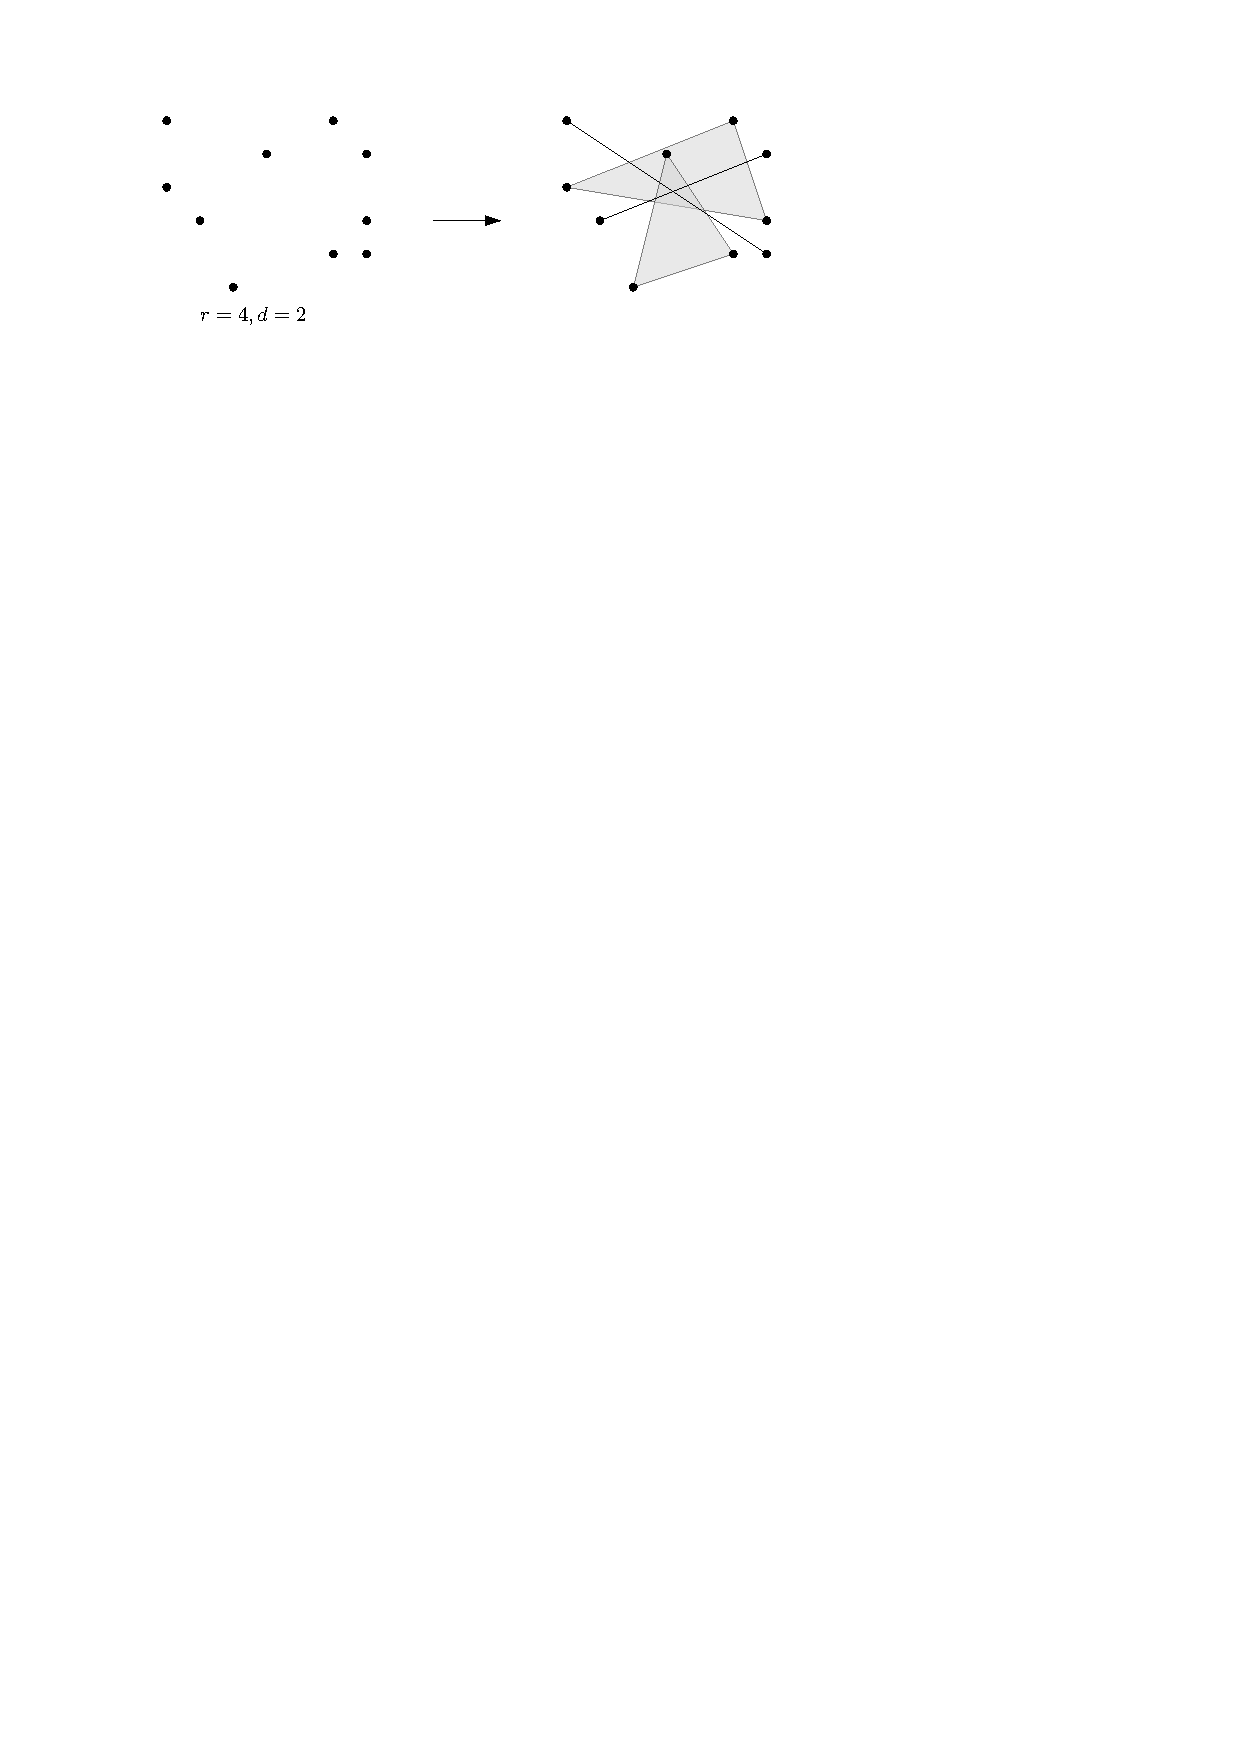
\includegraphics[scale=1]{fig1-Tverberg}}
		\caption{An example of a Tverberg partition.  The partition is not unique.}
	\end{figure}
	
	More formally, given $X\subset \rr^d$ of $(r-1)(d+1)+1$ points, there is a partition $X=X_1\cup \dots \cup X_r$ such that $\bigcap_{j=1}^r \conv X_j \ne \emptyset$. Such a partition is called a
	\textit{Tverberg partition}. The number of points in this result is optimal, as a dimension-counting argument shows. In fact, if $X$ is in general enough position and in the partition $X=X_1\cup \ldots \cup X_r$ we have $1\le |X_j|\le d+1$ for every $j$, then $\bigcap_{j=1}^r \aff X_j$ is a single point if $|X|= (r-1)(d+1)+1$, and is empty if $|X|\le (r-1)(d+1)$.
	
	% The case $r=2$ was proved first by Radon, as a lemma in his proof of Helly's theorem.
	
	The last decade has seen an impressive sequence of results around Tverberg's theorem.  The purpose of this survey is to give a broad overview of  the current state of the field and point out key open problems.  Other surveys covering different aspects of Tverberg's theorem can be found in \cite{Eckhoff:1979bi, Eck93survey, Matousek:2002td, BBZ17survey, de2017discrete, BZ17}.
	
	The paper is organized as follows.  In sections \ref{section-topological} and \ref{section-colored} we describe the topological and colorful versions of Tverberg's theorem, which have received the most attention in recent years.  In sections \ref{section-intersection} and \ref{section-universal} we discuss a large number of variations and conjectures around Tverberg's theorem.  In Section \ref{section-applications} we describe some applications of Tverberg's theorem.  Finally, in Section \ref{section-spaces} we present Tverberg-type results where the settings have changed dramatically, such as Tverberg for convexity spaces or quantitative versions.  In that last section, we focus mostly on results which are related to geometry.
	
	\subsection{Interlude: a short history of Tverberg's theorem}
	An early predecessor of Tverberg's theorem is Radon's lemma from 1921 \cite{Radon:1921vh, Eckhoff:1979bi}. Radon used it in his proof of Helly's theorem. It says that \textit{any set $X$ of $d+2$ points in $\rr^d$ can be split into two sets whose convex hulls intersect}. So it is the case $r=2$ of Tverberg's theorem. Its proof is simple: the $d+2$ vectors in $X$ have a nontrivial affine dependence $\sum_{x \in X}\al(x)x=0$ and  $\sum_{x \in X}\al(x)=0$. The sets $X_1=\{x \in X: \al(x)\ge 0\}$ and $X_2=\{x \in X: \al(x) < 0\}$ form a partition of $X$ and their convex hulls intersect, as one can easily check.
	
	Another result linked to this theorem is Rado's centerpoint theorem.  This states that \textit{for any set $X$ of $n$ points in $\rr^d$, there is a point $p$ such that any closed half-space that contains $p$ also contains at least $\left\lceil \frac{n}{d+1}\right\rceil$ points of $X$}. The standard proof of this result uses Helly's theorem. Tverberg's theorem implies it in few lines: setting $r=\left\lceil \frac{n}{d+1}\right\rceil$, there is a partition of $X$ into $r$ parts $X_1,\ldots,X_r$ and a point $p\in \rr^d$ such that $p \in \bigcap_{j=1}^r \conv X_j$. Then $p$ is a centerpoint of $X$: every closed halfspace containing $p$ contains at least one point from each $X_j$.
	
	In a paper entitled ``On $3N$ points in a plane'' Birch~\cite{Birch:1959} proves that any $3N$ points in the plane determine $N$ triangles that have a point in common. His motivation was the (planar) centerpoint theorem. Actually, he proves more, namely the case $d=2$ of Tverberg's theorem and states the general case as a conjecture.
	
	Tverberg's original motivation was also the centerpoint theorem and he learned about Birch's result and conjecture only later. He proved it first for $d=3$ in 1963, and in full generality in 1964.  Here is, in his own words, how he found the proof:  ``I recall that the weather was bitterly cold in Manchester. I awoke very early one morning shivering, as the electric heater in the hotel room had gone off, and I did not have an extra shilling to feed the meter. So, instead of falling back to sleep, I reviewed the problem once more, and then the solution dawned on me!'' \cite{tve:recollections}.
	
	\section{Topological versions}\label{section-topological}
	
	\section{Colorful versions}\label{section-colored}
	
	\section{The structure of Tverberg partitions}\label{section-intersection}
	
	\section{Universal Tverberg partitions}\label{section-universal}
	
	\section{Applications of Tverberg's theorem}\label{section-applications}
	
	\section{Tverberg-type results in distinct settings}\label{section-spaces}
	
	\bibliographystyle{alpha}
	\bibliography{references} % see references.bib for bibliography management
	
\end{document}
